\chapter{Time Evolution, Interference, and the Schr\"odinger Equation}

This lecture sets out to do one thing: to begin the serious study of how quantum systems change with time. But Susskind does not begin by writing down the Schr\"odinger equation. He first backs up, gives a very compressed reminder of classical evolution, and isolates the one structural fact that matters for what follows: the Hamiltonian generates motion. From there the lecture moves in a tight sequence. We pass from preserved relations between states to unitary evolution, from infinitesimal evolution to a Hermitian generator, from that generator to the abstract Schr\"odinger equation, and then immediately into examples where the phases produced by time evolution become measurable through interference. These notes follow Leonard Susskind's lecture, with supporting board-frame evidence curated by LazyingArt LLC and Video2Book.

\section{From Classical Flow To The Hamiltonian}

The opening classical recap is deliberately brief. For a discrete system, time evolution amounts to jumps from one state to another, and those jumps naturally come in sampled time intervals. Continuous time becomes natural only for systems with continuous variables. A particle moving on a line is the simplest example: at each instant it has a position $x$ and a momentum $p$, and its motion is described not by hops on a finite graph but by a flow in phase space.

The Hamiltonian is the object that describes that flow. For a particle on a line it is a function of $x$ and $p$, and in the standard mechanical example it takes the form
\begin{equation}
H(x,p)=\frac{p^2}{2m}+U(x).
\end{equation}
In the board frame the equality sign and punctuation are not completely secure, but the printed expression is the natural completion of the visible formula.

\begin{figure}[h]
\centering

\includegraphics[width=0.62\textwidth]{lecture_08_figure_02.png}
\par
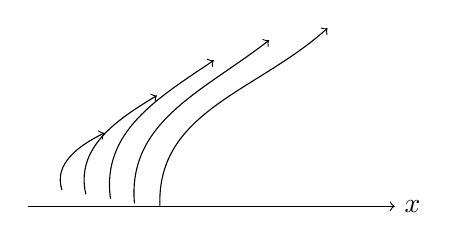
\begin{tikzpicture}[scale=0.95]
\draw[->] (0,0) -- (4.9,0) node[right] {$x$};
\draw[->] (0.45,0.22) to[out=108,in=206] (1.02,0.98);
\draw[->] (0.77,0.16) to[out=103,in=211] (1.72,1.48);
\draw[->] (1.10,0.10) to[out=98,in=214] (2.48,1.95);
\draw[->] (1.42,0.04) to[out=95,in=218] (3.22,2.22);
\draw[->] (1.76,0.00) to[out=92,in=222] (4.00,2.38);
\end{tikzpicture}
\caption{Classical Hamiltonian and flow-line sketch. The redraw is intentionally conservative: the lecture frame clearly secures the curved flow and the $x$ label, but not a full axis system.}
\end{figure}

The flow is determined by Hamilton's equations,
\begin{align}
\dot x &= \frac{\partial H}{\partial p},
&
\dot p &= -\frac{\partial H}{\partial x}.
\end{align}
In particular, for the Hamiltonian above we have $\partial H/\partial p=p/m$, which is the velocity, while $-\partial H/\partial x$ is the force.

If $f(x,p)$ is any observable quantity, its time derivative is obtained from the chain rule:
\begin{align}
\dot f
&=
\frac{\partial f}{\partial x}\dot x
+
\frac{\partial f}{\partial p}\dot p \\
&=
\frac{\partial f}{\partial x}\frac{\partial H}{\partial p}
-
\frac{\partial f}{\partial p}\frac{\partial H}{\partial x}.
\end{align}
This combination is the Poisson bracket with the Hamiltonian:
\begin{equation}
\dot f=\{f,H\}_{\mathrm{PB}}.
\end{equation}

Susskind immediately compresses all of this into the sentence that matters: the Hamiltonian generates time evolution. The Poisson-bracket formalism is not being reviewed for its own sake. It is there to prepare the quantum replacement.

\section{From Preserved Relations To Unitary Evolution}

The pivot is sharp. Classical mechanics, Susskind says, always felt more obscure than it should have; something simpler must underlie it, and what underlies it is quantum mechanics. So instead of asking for trajectories in phase space, we ask what quantum time evolution preserves.

The answer is: the relations between states are preserved. If two states are orthogonal, they remain orthogonal. If they overlap by a certain amount, that overlap is preserved. One may picture the whole space of states as rotating, but without changing the angles between vectors.

Suppose a state $|A\rangle$ evolves over a time interval $T$. We write
\begin{equation}
|A\rangle \mapsto U(T)|A\rangle.
\end{equation}
If a second state $|B\rangle$ evolves over the same interval, then
\begin{equation}
|B\rangle \mapsto U(T)|B\rangle,
\qquad
\langle B| \mapsto \langle B|U^\dagger(T).
\end{equation}
Now require that the inner product be preserved:
\begin{equation}
\langle B|A\rangle
=
\langle B|U^\dagger(T)U(T)|A\rangle
\end{equation}
for arbitrary states $|A\rangle$ and $|B\rangle$. Therefore
\begin{equation}
U^\dagger(T)U(T)=1.
\end{equation}
So time evolution is governed by a unitary operator.

In the lecture this is presented almost as the whole principle in one line: things which are orthogonal stay orthogonal. That is enough to force unitarity.

It is useful now to write the evolution law in the form used throughout the rest of the lecture:
\begin{equation}
|\psi(t+T)\rangle = U(T)|\psi(t)\rangle.
\end{equation}
This says nothing more mysterious than that if we want to push a state ahead by an amount of time $T$, we do it by acting on it with the evolution operator $U(T)$.

\section{Infinitesimal Time Steps And The Hermitian Generator}

Once time evolution is known to be unitary for finite intervals, the next natural question is local: what is $U(\epsilon)$ for a very short interval $\epsilon$? Since no evolution at all should do nothing, we must have
\begin{equation}
U(0)=1.
\end{equation}
Therefore the leading small-$\epsilon$ form must be
\begin{equation}
U(\epsilon)=1-\frac{i\epsilon}{\hbar}H+O(\epsilon^2).
\end{equation}
At this stage the notation is partly anticipatory. The factors of $i$ and $\hbar$ are chosen so that the operator $H$ will later be recognized as the Hamiltonian. Susskind is explicit about this: the formula has been written in a way that will eventually make contact with classical mechanics.

A student immediately raises the classical-limit question: if $\hbar$ appears in the denominator, what can it mean to let $\hbar\to 0$? The answer is that the meaningful quantity is not $\hbar$ in isolation, but the dimensionless ratio $\epsilon H/\hbar$, or more broadly an action measured in units of $\hbar$. At this stage the placement of $\hbar$ is bookkeeping; later it will be precisely what allows $H$ to have a sensible classical meaning.

Now take the Hermitian conjugate:
\begin{equation}
U^\dagger(\epsilon)=1+\frac{i\epsilon}{\hbar}H^\dagger+O(\epsilon^2).
\end{equation}
Imposing unitarity to first order,
\begin{align}
1
&=
U^\dagger(\epsilon)U(\epsilon) \\
&=
\left(1+\frac{i\epsilon}{\hbar}H^\dagger\right)
\left(1-\frac{i\epsilon}{\hbar}H\right)
+O(\epsilon^2) \\
&=
1+\frac{i\epsilon}{\hbar}(H^\dagger-H)+O(\epsilon^2),
\end{align}
so the first-order term must vanish:
\begin{equation}
H^\dagger=H.
\end{equation}

That is the first genuinely new conclusion. The generator of infinitesimal time evolution must be Hermitian. It follows that it is an observable: it has real eigenvalues and an orthonormal basis of eigenvectors. Only after deriving that fact does Susskind give the operator its physical name. We call it the Hamiltonian, and we call its eigenvalues energies. He is careful about the logical order: we are not yet proving that this is the same energy as in classical mechanics, only that this is the observable whose eigenvalues deserve the name.

\section{The Abstract Schr\"odinger Equation}

Now we turn the infinitesimal update rule into a differential equation. Starting from
\begin{equation}
|\psi(t+\epsilon)\rangle
=
\left(1-\frac{i\epsilon}{\hbar}H\right)|\psi(t)\rangle,
\end{equation}
we bring the identity term to the left:
\begin{equation}
|\psi(t+\epsilon)\rangle-|\psi(t)\rangle
=
-\frac{i\epsilon}{\hbar}H|\psi(t)\rangle.
\end{equation}
Dividing by $\epsilon$ and letting $\epsilon\to 0$ gives
\begin{equation}
\frac{\partial}{\partial t}|\psi\rangle
=
-\frac{i}{\hbar}H|\psi\rangle.
\end{equation}
Multiplying by $i\hbar$, we obtain the canonical form
\begin{equation}
i\hbar\,\frac{\partial}{\partial t}|\psi\rangle=H|\psi\rangle.
\end{equation}

This is the abstract Schr\"odinger equation. Susskind pauses at exactly this point to stress what it is and what it is not. It is the general law of quantum time evolution. It is not yet the original wave equation Schr\"odinger wrote down for a particle moving in space. In this abstract form, it applies to any quantum system whatever, provided we know its Hamiltonian.

The lecture later reuses the same equation in the simplified $\hbar=1$ convention. The board snapshot below captures that stripped-down ket form:
\begin{figure}[h]
\centering

\includegraphics[width=0.42\textwidth]{lecture_08_figure_04.png}
\caption{Ket form of the Schr\"odinger equation in the lecture's temporary $\hbar=1$ convention.}
\end{figure}

The cleaned board equation is
\begin{equation}
|\dot\psi\rangle=-iH|\psi\rangle,
\end{equation}
which is exactly the same statement as the previous equation with $\hbar$ suppressed.

At this point the lecture takes a deliberate turn. A differential equation only earns its keep when it predicts the future. So Susskind asks how this formalism is actually used.

\section{Polarization Example: Energy Eigenstates And Phase Evolution}

The first worked example returns to the familiar two-state system of photon polarization. Imagine a material in which a photon of fixed wavelength has different energies depending on its polarization. Let the $x$ polarization have energy $E_1$ and the $y$ polarization have energy $E_2$. Then the Hamiltonian has the basis states $|x\rangle$ and $|y\rangle$ as eigenvectors:
\begin{equation}
H|x\rangle=E_1|x\rangle,
\qquad
H|y\rangle=E_2|y\rangle.
\end{equation}

\begin{figure}[h]
\centering

\includegraphics[width=0.74\textwidth]{lecture_08_figure_03.png}
\caption{Polarization energy eigenstates and time-dependent state. The lower state vector is partly blocked in the board frame, so the printed form follows the transcript rather than the image alone.}
\end{figure}

A general state of polarization is written as
\begin{equation}
|\psi(t)\rangle=
\begin{pmatrix}
\alpha(t)\\
\beta(t)
\end{pmatrix},
\end{equation}
where $\alpha(t)$ is the amplitude for $x$ polarization and $\beta(t)$ is the amplitude for $y$ polarization.

From this point on in the live lecture Susskind temporarily sets $\hbar=1$. We will restore $\hbar$ in the printed formulas, but it is worth remembering that the corresponding board equations are written in the simplified convention.

In the $(|x\rangle,|y\rangle)$ basis the Hamiltonian is diagonal:
\begin{equation}
H=
\begin{pmatrix}
E_1 & 0\\
0 & E_2
\end{pmatrix}.
\end{equation}
The lecture briefly writes the diagonal entries in the wrong order and then corrects them; the matrix above is the corrected form.

Now apply the Schr\"odinger equation:
\begin{equation}
i\hbar\frac{d}{dt}
\begin{pmatrix}
\alpha\\
\beta
\end{pmatrix}
=
\begin{pmatrix}
E_1 & 0\\
0 & E_2
\end{pmatrix}
\begin{pmatrix}
\alpha\\
\beta
\end{pmatrix}.
\end{equation}
Because the Hamiltonian is diagonal, the two amplitudes do not mix. We simply get
\begin{equation}
i\hbar\,\dot\alpha=E_1\alpha,
\qquad
i\hbar\,\dot\beta=E_2\beta.
\end{equation}
These are the simplest possible first-order differential equations, and their solutions are pure exponentials:
\begin{equation}
\alpha(t)=\alpha(0)e^{-iE_1 t/\hbar},
\qquad
\beta(t)=\beta(0)e^{-iE_2 t/\hbar}.
\end{equation}
Therefore
\begin{equation}
|\psi(t)\rangle=
\begin{pmatrix}
\alpha(0)e^{-iE_1 t/\hbar}\\
\beta(0)e^{-iE_2 t/\hbar}
\end{pmatrix}.
\end{equation}

Susskind now asks the obvious experimental question. What happens if we measure the polarization in the $x/y$ basis itself? The answer is almost perversely simple:
\begin{equation}
|\alpha(t)|^2=|\alpha(0)|^2,
\qquad
|\beta(t)|^2=|\beta(0)|^2.
\end{equation}
The phases drop out. At first sight it looks as if time evolution has done nothing at all.

\subsection{Question \& Answer}

\paragraph{Question.}
If the two components only pick up phases, and if the $x/y$ probabilities do not change, has anything observable happened?

\paragraph{Answer.}
Yes, but we have to look in the right basis. The phases disappear only when we measure in the basis in which the Hamiltonian is diagonal. If we rotate the measurement basis, the relative phase becomes visible through interference.

Take the $45^\circ$ polarization state
\begin{equation}
|/\rangle
=
\frac{1}{\sqrt2}
\begin{pmatrix}
1\\
1
\end{pmatrix}.
\end{equation}
The amplitude to pass a $45^\circ$ polarizer is
\begin{equation}
\langle /|\psi(t)\rangle
=
\frac{1}{\sqrt2}
\left(
\alpha(0)e^{-iE_1 t/\hbar}
+
\beta(0)e^{-iE_2 t/\hbar}
\right).
\end{equation}

Now specialize to the experimental arrangement emphasized in the lecture: the photon first passes through a $45^\circ$ polarizer, so at $t=0$ we have
\begin{equation}
\alpha(0)=\beta(0)=\frac{1}{\sqrt2}.
\end{equation}
Then the amplitude becomes
\begin{equation}
A_{/}(t)
=
\frac12
\left(
e^{-iE_1 t/\hbar}
+
e^{-iE_2 t/\hbar}
\right).
\end{equation}
The corresponding probability is
\begin{align}
P(t)
&=
|A_{/}(t)|^2 \\
&=
\frac14
\left(
e^{-iE_1 t/\hbar}+e^{-iE_2 t/\hbar}
\right)
\left(
e^{iE_1 t/\hbar}+e^{iE_2 t/\hbar}
\right) \\
&=
\frac14
\left(
2
+
e^{i(E_2-E_1)t/\hbar}
+
e^{-i(E_2-E_1)t/\hbar}
\right).
\end{align}
Defining
\begin{equation}
\Delta E=E_2-E_1,
\end{equation}
we arrive at
\begin{equation}
P(t)=\frac12\left(1+\cos\frac{\Delta E\,t}{\hbar}\right).
\end{equation}

This is the real payoff of the example. The state has certainly changed. The relative phase between the two components becomes a physically measurable oscillation when we project onto the rotated basis. At $t=0$ we get $P(0)=1$, as we should: two parallel $45^\circ$ polarizers with no time evolution between them transmit with certainty. Later the probability can fall all the way to zero. That means the photon certainly does \emph{not} pass the second polarizer in the original direction. The lecture interprets this physically as a rotation of the linear polarization as the photon moves downstream through the material.

The central point is broader than this one example. Only the energy difference matters. If we add the same constant to both energies, then the state acquires only an overall phase, and that common phase cancels from every probability. Thus physics depends on $\Delta E$, not on the arbitrary zero of energy.

This also resolves the student's worry that the choice of $x$ and $y$ seems arbitrary. It is the material itself that picks preferred axes. When our measurement basis is aligned with those axes, the Hamiltonian is diagonal and the probabilities in that basis stay fixed. When the basis is misaligned, the relative phase shows up as rotation and interference.

\section{Expectation Values, Commutators, And Conserved Quantities}

Before taking a break, Susskind does one more thing. He steps back from the polarization example and asks for a general theorem. Suppose $K$ is some observable. How does its expectation value
\begin{equation}
\langle K\rangle=\langle\psi|K|\psi\rangle
\end{equation}
change with time?

\begin{figure}[h]
\centering

\includegraphics[width=0.62\textwidth]{lecture_08_figure_05.png}
\caption{Product-rule step toward the commutator formula. The board image secures the intermediate structure, while the full displayed formula below is reconstructed from the transcript.}
\end{figure}

The first step is utterly ordinary: the time derivative of a product is the sum of two terms. Since $K$ itself is held fixed, only the bra and ket change:
\begin{equation}
\frac{d}{dt}\langle\psi|K|\psi\rangle
=
\langle\psi|K|\dot\psi\rangle
+
\langle\dot\psi|K|\psi\rangle.
\end{equation}
Now use the Schr\"odinger equation for the ket and its Hermitian conjugate for the bra:
\begin{equation}
|\dot\psi\rangle=-\frac{i}{\hbar}H|\psi\rangle,
\qquad
\langle\dot\psi|=\frac{i}{\hbar}\langle\psi|H.
\end{equation}
Substituting, we find
\begin{align}
\frac{d}{dt}\langle K\rangle
&=
-\frac{i}{\hbar}\langle\psi|KH|\psi\rangle
+\frac{i}{\hbar}\langle\psi|HK|\psi\rangle \\
&=
-\frac{i}{\hbar}\langle\psi|(KH-HK)|\psi\rangle.
\end{align}
With the convention
\begin{equation}
[K,H]=KH-HK,
\end{equation}
the result becomes
\begin{equation}
\frac{d}{dt}\langle K\rangle
=
-\frac{i}{\hbar}\langle[K,H]\rangle.
\end{equation}

That is the general law. In the lecture Susskind is pleased by how short the derivation is. Time-differentiate the sandwich, use the ket equation once and the bra equation once, and the opposite signs conspire to produce a commutator.

This is the direct quantum analog of the classical rule
\begin{equation}
\dot f=\{f,H\}_{\mathrm{PB}}.
\end{equation}
In both theories, it is the Hamiltonian that controls time evolution. In classical mechanics the bracket is the Poisson bracket; in quantum mechanics it is the commutator.

\begin{proposition}
If an observable $K$ commutes with the Hamiltonian, then its expectation value is conserved:
\begin{equation}
[K,H]=0
\qquad \Longrightarrow \qquad
\frac{d}{dt}\langle K\rangle=0.
\end{equation}
\end{proposition}

\begin{proof}
If $[K,H]=0$, then the right-hand side of
\[
\frac{d}{dt}\langle K\rangle
=
-\frac{i}{\hbar}\langle[K,H]\rangle
\]
vanishes.
\end{proof}

Susskind remarks that one can prove a stronger statement about the full probability distribution, but he does not pursue it here. For present purposes the expectation-value theorem is enough. In particular, the Hamiltonian commutes with itself, so the Hamiltonian is conserved. Since the Hamiltonian is the energy, energy conservation appears here not as an additional postulate, but as a direct consequence of the formalism.

\section{Particle On A Line And The Free-Particle Schr\"odinger Equation}

Only after the two-state example and the commutator theorem does the lecture turn to Schr\"odinger's original setting: a particle moving on a line. The state can be described by a wave function $\psi(x,t)$, or equivalently by its Fourier transform $\tilde\psi(p,t)$. Nothing fundamental has changed. We have only traded an abstract ket for its coordinate representation. Functions of $x$ are vectors too.

The rule of time evolution is the same rule as before:
\begin{equation}
i\hbar\,\frac{\partial}{\partial t}\psi(x,t)=H\psi(x,t).
\end{equation}
What remains is to identify the Hamiltonian for a free particle.

We know that in classical mechanics the energy is
\begin{equation}
E=\frac{p^2}{2m}.
\end{equation}
Susskind is careful here: classical mechanics does not prove the quantum Hamiltonian. At best it suggests a guess. The natural guess is
\begin{equation}
\hat H=\frac{\hat p^2}{2m}.
\end{equation}
The momentum operator is
\begin{equation}
\hat p=-i\hbar\frac{\partial}{\partial x}.
\end{equation}
Therefore
\begin{equation}
\hat H
=
\frac{1}{2m}
\left(-i\hbar\frac{\partial}{\partial x}\right)^2
=
-\frac{\hbar^2}{2m}\frac{\partial^2}{\partial x^2}.
\end{equation}

The live lecture then goes through exactly the kind of sign-and-factor tangle one expects in real time, notices a missing $\hbar$, loses track of a minus sign, and finally decides to do the calculation over carefully. The cleaned result is the standard free-particle Schr\"odinger equation:
\begin{equation}
i\hbar\,\frac{\partial}{\partial t}\psi(x,t)
=
-\frac{\hbar^2}{2m}\frac{\partial^2}{\partial x^2}\psi(x,t).
\end{equation}

Now solve it for a momentum eigenstate. We look for a wave function that remains an eigenfunction of momentum at every instant:
\begin{equation}
\psi_p(x,t)=f(t)e^{ipx/\hbar}.
\end{equation}
Differentiating with respect to time hits only $f(t)$:
\begin{equation}
\frac{\partial\psi_p}{\partial t}
=
\dot f(t)e^{ipx/\hbar}.
\end{equation}
Differentiating twice with respect to $x$ hits only the exponential:
\begin{equation}
\frac{\partial^2\psi_p}{\partial x^2}
=
-\frac{p^2}{\hbar^2}f(t)e^{ipx/\hbar}.
\end{equation}
Substituting into the Schr\"odinger equation, we get
\begin{equation}
i\hbar\,\dot f(t)e^{ipx/\hbar}
=
\frac{p^2}{2m}f(t)e^{ipx/\hbar}.
\end{equation}
Cancel the common factor $e^{ipx/\hbar}$:
\begin{equation}
i\hbar\,\dot f=\frac{p^2}{2m}f,
\qquad\text{or}\qquad
\dot f=-\frac{i p^2}{2m\hbar}f.
\end{equation}
Hence
\begin{equation}
f(t)=e^{-ip^2 t/(2m\hbar)}
\end{equation}
up to normalization, and therefore
\begin{equation}
\psi_p(x,t)
=
\exp\!\left[\frac{i}{\hbar}\left(px-\frac{p^2}{2m}t\right)\right]
\end{equation}
up to an overall constant factor.

Once again the time dependence is a pure phase. For a single momentum eigenstate there is no change in the momentum probability distribution; the state simply accumulates the phase appropriate to its energy. The lecture closes by pointing out the simple exercise
\begin{equation}
[p,H]=0
\qquad\text{for}\qquad
H=\frac{p^2}{2m},
\end{equation}
so momentum is conserved for the free particle. The next natural questions, which Susskind leaves for later, concern what happens for superpositions: does the probability for a given momentum change, and what about the probability for a given position?

\section{Summary}

The lecture has unfolded in a very specific order. We began with classical flow only long enough to isolate the structural role of the Hamiltonian. We then replaced phase-space flow by preservation of inner products, and from that preservation recovered unitary time evolution. Studying an infinitesimal time step forced the generator to be Hermitian, and from the infinitesimal update rule we obtained the abstract Schr\"odinger equation.

The polarization example then showed why the equation matters. A diagonal Hamiltonian makes the individual components pick up phases, and at first sight those phases seem invisible. But once we rotate the measurement basis, the relative phase becomes measurable through interference, and only energy differences survive. From there the commutator law for expectation values follows almost at once, together with the criterion for conserved quantities. Finally, by replacing kets with wave functions and guessing the Hamiltonian from the classical free-particle energy, we recover Schr\"odinger's original differential equation and its plane-wave solutions. The whole lecture is guided by one persistent idea: the Hamiltonian is the generator of time evolution.